\chapter{Implementacija i korisničko sučelje}
		
		
		\section{Korištene tehnologije i alati}
		
		Za izradu web aplikacije korištene su brojne tehnologije koje su pomogle u izradi backend i frontend dijela aplikacije. Razvojna okolina koja se koristila za backend dio je \underline{IDE Eclipse}\footnote{\url{https://www.eclipse.org/}}. Eclipse IDE je programska razvojna okolina pisana u Javi razvijena od tvrtke Eclipse Foundation, a može se koristiti za razvoj aplikacija u raznim programskim jezicima (Java, C, C++, Perl, Python,...). Za izradu backenda koristio se programski jezik \underline{Java}\footnote{\url{https://www.java.com/}} te tehnologije \underline{Java Servleti}\footnote{\url{https://www.oracle.com/technetwork/java/javaee/servlet/index.html}} i \underline{JSP}\footnote{\url{https://www.oracle.com/technetwork/java/}} (Java Servet Pages). Za smještaj servleta korišten je \underline{Apache Tomcat}\footnote{\url{https://tomcat.apache.org/}}. Apache Tomcat je open source Web poslužitelj koji implementira nekoliko Java EE specifikacija kao što su Java Servlet, JSP (Java Servlet Pages), Java EL (Java Expression Language). Može se koristiti kao samostalan web server ili kao poslužitelj za servlete i Java Server Pages (JSP) integriran s nekim drugim web poslužiteljem.
		Kao web poslužitelj koristi se \underline{Windows Server}\footnote{\url{https://www.microsoft.com/en-us/cloud-platform/windows-server}} virtualna mašina podignuta preko servisa \underline{Microsoft Azure}\footnote{\url{https://portal.azure.com/}} na kojemu su instalirani svi servisi koji podupiru rad web aplikacije i baze podataka. Baza podataka pokrenuta je pomoću sustava \underline{PostgreSQL}\footnote{\url{https://www.postgresql.org/}}. 
		
		Mobilna aplikacija je izgrađena u programskom jeziku Java koristeći razvojnu okolinu \underline{Android studio}\footnote{\url{https://developer.android.com/studio/index.html}}. Mobilna aplikacija spaja se na RESTful dio web poslužitelja preko kojeg vrši prijavu u sustav i dohvaćanje podataka. Dizajna Android aplikacije postignut je korištenjem sustava \underline{Adobe XD}\footnote{\url{https://www.adobe.com/products/xd.html}} i \underline{Google Material Design}\footnote{\url{https://www.material.io/}} kao vizualnim jezikom.
		
		 Pomoću alata \underline{Astah Proffesional}\footnote{\url{https://http://astah.net/editions/professional}} nacrtani su UML dijagrami, a kao sustav za upravljanje izvornim kodom korišten je \underline{Git}\footnote{\url{https://git-scm.com/}}. Udaljeni repozitorij projekta je dostupan na web platformi
		\underline{GitLab}\footnote{\url{https://www.gitlab.com/}}. Članovi tima komunicirali su korištenjem aplikacije \underline{Slack}\footnote{\url{https://www.slack.com/}}.
		
		
	\newpage
		\section{Ispitivanje programskog rješenja}
			
			\textbf{\textit{dio 2. revizije}}\\
			
			 \textit{U ovom poglavlju je potrebno opisati provedbu ispitivanja implementiranih funkcionalnosti na razini komponenti i na razini cijelog sustava s prikazom odabranih ispitnih slučajeva. Studenti trebaju ispitati temeljnu funkcionalnost i rubne uvjete..}
	
			
			\subsection{Ispitivanje komponenti (JUnit testiranje)}
			\begin{figure}[H]
				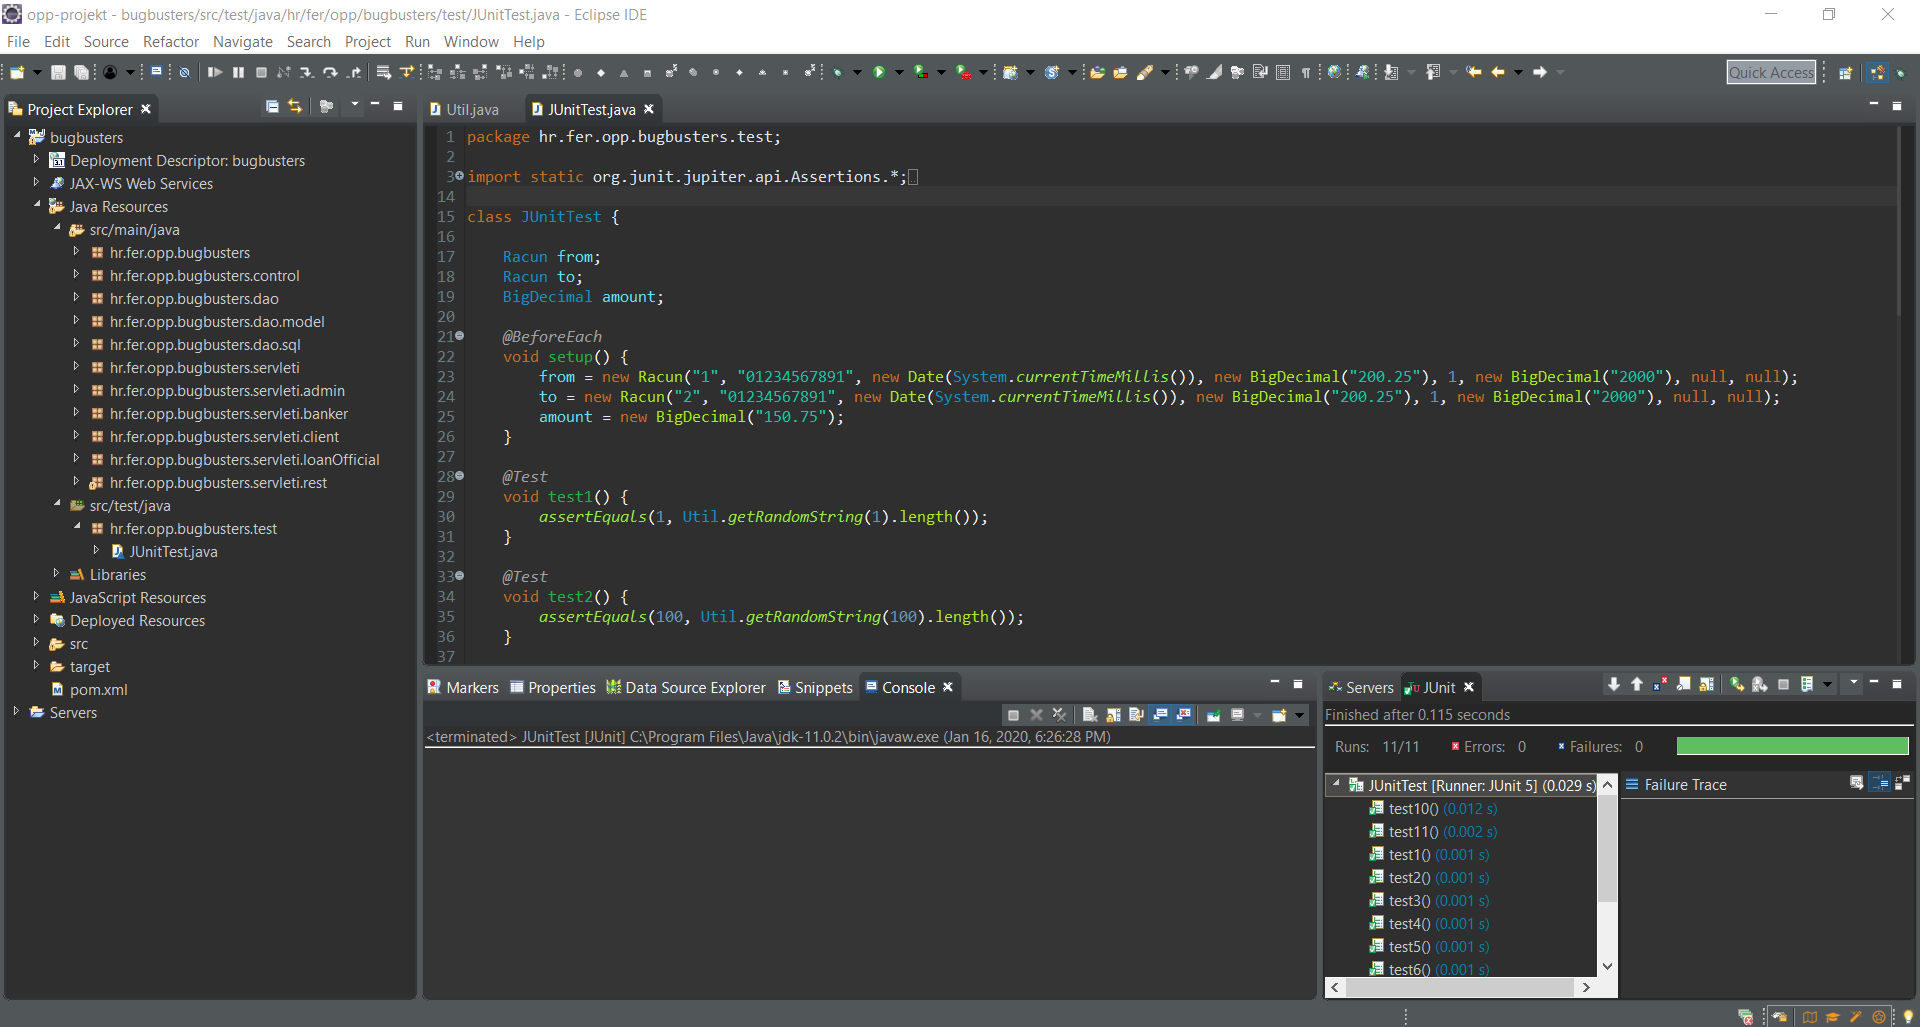
\includegraphics[scale=0.4]{Slike/junit.png}
				\centering
				\caption{JUnit testovi}
				\label{fig:dijagram}
			\end{figure}
		
		\begin{lstlisting}[language=Java]
package hr.fer.opp.bugbusters.test;

import static org.junit.jupiter.api.Assertions.*;

import java.math.BigDecimal;
import java.sql.Date;

import org.junit.jupiter.api.BeforeEach;
import org.junit.jupiter.api.Test;

import hr.fer.opp.bugbusters.control.Util;
import hr.fer.opp.bugbusters.control.Util.TransakcijaCollection;
import hr.fer.opp.bugbusters.dao.model.Racun;

class JUnitTest {

Racun from;
Racun to;
BigDecimal amount;

@BeforeEach
void setup() {
	from = new Racun("1", "01234567891", new Date(System.currentTimeMillis()), new BigDecimal("200.25"), 1, new BigDecimal("2000"), null, null);
	to = new Racun("2", "01234567891", new Date(System.currentTimeMillis()), new BigDecimal("200.25"), 1, new BigDecimal("2000"), null, null);
	amount = new BigDecimal("150.75");
}

@Test
void test1() {
	assertEquals(1, Util.getRandomString(1).length());
}

@Test
void test2() {
	assertEquals(100, Util.getRandomString(100).length());
}

@Test
void test3() {
	assertThrows(IllegalArgumentException.class, () -> Util.getRandomString(0));
}

@Test
void test4() {
	assertThrows(IllegalArgumentException.class, () -> Util.getRandomString(-10));
}

@Test
void test5() {
	assertThrows(NullPointerException.class, () -> Util.doTransaction(null, to, amount));
}

@Test
void test6() {
	assertThrows(NullPointerException.class, () -> Util.doTransaction(from, null, amount));
}

@Test
void test7() {
	assertThrows(NullPointerException.class, () -> Util.doTransaction(from, to, null));
}

@Test
void test8() {
	assertThrows(IllegalArgumentException.class, () -> Util.doTransaction(from, to, new BigDecimal("2500")));
}

@Test
void test9() {
	assertThrows(IllegalArgumentException.class, () -> Util.doTransaction(from, to, new BigDecimal("0")));
}

@Test
void test10() {
	assertThrows(IllegalArgumentException.class, () -> Util.doTransaction(from, to, new BigDecimal("-1")));
}

@Test
void test11() {
	TransakcijaCollection tc = Util.doTransaction(from, to, amount);
	assertEquals(new BigDecimal("49.50"), tc.from.getStanje());
	assertEquals(new BigDecimal("351.00"), tc.to.getStanje());
}

}
		\end{lstlisting}
			
			
			
			\subsection{Ispitivanje sustava}
			
			 \textit{Potrebno je provesti i opisati ispitivanje sustava koristeći radni okvir Selenium\footnote{\url{https://www.seleniumhq.org/}}. Razraditi \textbf{minimalno 4 ispitna slučaja} u kojima će se ispitati redovni slučajevi, rubni uvjeti te poziv funkcionalnosti koja nije implementirana/izaziva pogrešku kako bi se vidjelo na koji način sustav reagira kada nešto nije u potpunosti ostvareno. Ispitni slučaj se treba sastojati od ulaza (npr. korisničko ime i lozinka), očekivanog izlaza ili rezultata, koraka ispitivanja i dobivenog izlaza ili rezultata.\\ }
			 
			 \textit{Izradu ispitnih slučajeva pomoću radnog okvira Selenium moguće je provesti pomoću jednog od sljedeća dva alata:}
			 \begin{itemize}
			 	\item \textit{dodatak za preglednik \textbf{Selenium IDE} - snimanje korisnikovih akcija radi automatskog ponavljanja ispita	}
			 	\item \textit{\textbf{Selenium WebDriver} - podrška za pisanje ispita u jezicima Java, C\#, PHP koristeći posebno programsko sučelje.}
			 \end{itemize}
		 	\textit{Detalji o korištenju alata Selenium bit će prikazani na posebnom predavanju tijekom semestra.}
			
			\eject 
		
		
		\section{Dijagram razmještaja}
			
			Slika prikazuje dijagram razmještaja u sustavu Internet bankarstva. Klijentsko računalo povezuje se s poslužiteljem putem Web preglednika putem http protokola. Android uređaji koriste Android aplikaciju za komunikaciju s poslužiteljem koja se također odvija http protokolom. Poslužiteljsko računalo sastoji se od Web poslužitelja na kojemu se nalazi Web aplikacija i od DB poslužitelja na kojemu se nalazi baza podataka.
			
			\begin{figure}[H]
				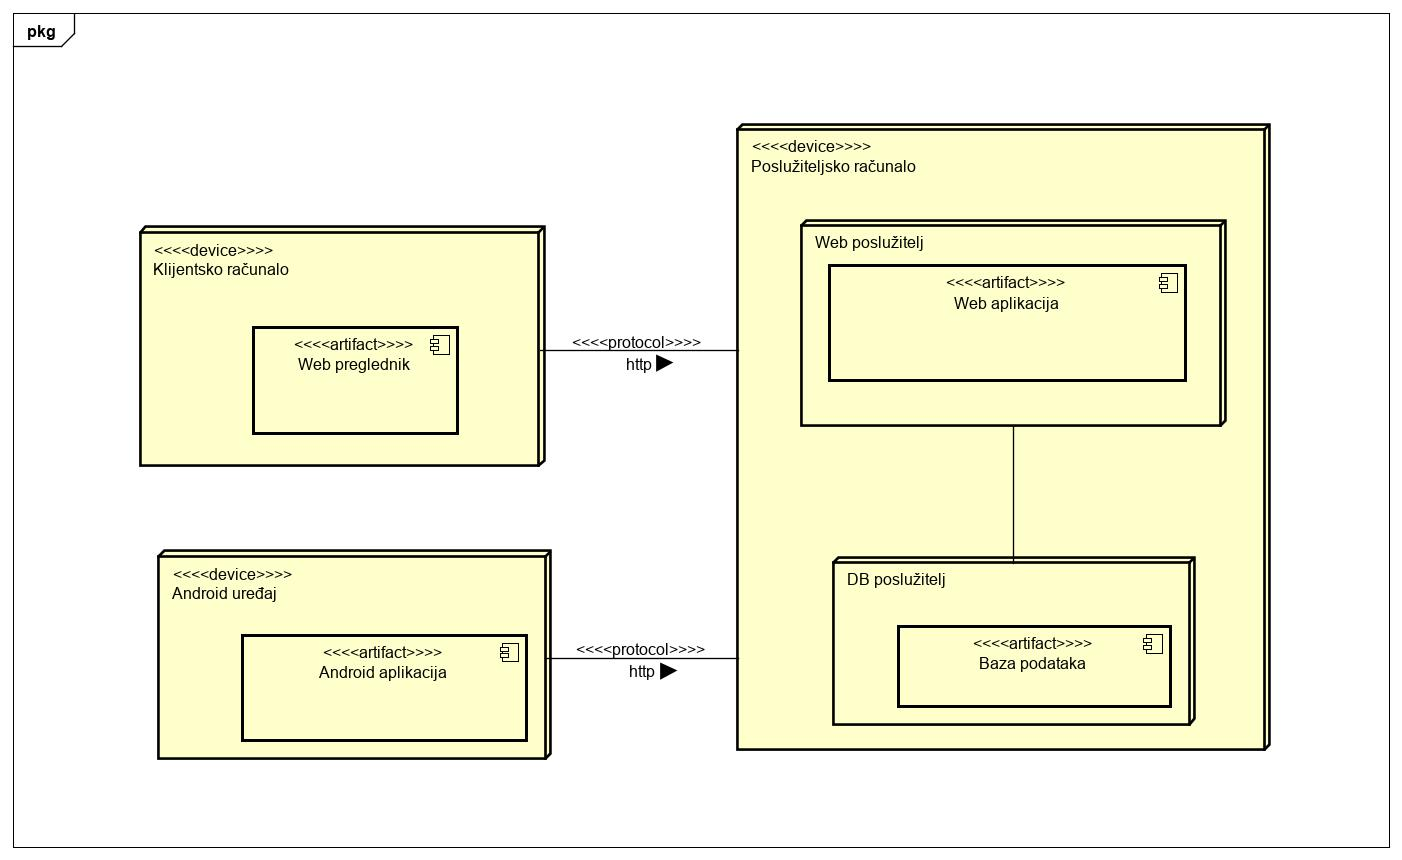
\includegraphics[scale=0.3]{Slike/dijagram_razmjestaja.jpg}
				\centering
				\caption{Dijagram razmještaja}
				\label{fig:dijagram}
			\end{figure}
		
		\newpage
		\section{Upute za puštanje u pogon}
		Web aplikacija Bugbusters banka puštena je u pogon pomoću servisa Microsoft Azure, gdje je i postavljen kod same aplikacije (backend i frontend). Aplikacija se pokreće pomoću web preglednika (npr. Google Chrome, Mozilla Firefox...) upisom adrese http://104.45.11.92/. Ovu adresu dodjelio je odabrani servis na kojem je aplikacija puštena u pogon. Upisom navedene adrese u web preglednik otvara se stranica za prijavu (engl. login) korisnika u aplikaciju. Za daljnji rad s aplikacijom potrebno je unijeti valjano korisničko ime i lozinku, a u slučaju prve prijave u sustav potrebno je unijeti OIB i korisnički ključ, te zatim promijeniti lozinku. Baza podataka pokrenuta je pomoću sustava PostgreSQL. Svi entiteti baze podataka opisani su java klasama čiji se kod nalazi unutar direktorija izvorniKod, točnije u poddirektoriju dao/model. Veza sa bazom podataka i mogućnost postavljanja upita nad bazom podataka ostvarena je pomoću klasa SQLConnectionProvider i SQLDAO. Ove klase služe kako bi se izradila funkcionalna baza podataka koju aplikacija može koristiti za svoj rad, tj. dohvaćanje, brisanje i izmjena podataka unutar baze podataka.\\
		
	 \textbf{Instalacija i konfiguracija poslužitelja baze podataka}
		
			Potrebno je preuzeti PostgreSQL (\underline{\url{https://www.postgresql.org/download/}}). Nakon pokretanja instalacije, kod odabira komponenti koje će se instalirati, obavezno odabrati PostgreSQL Server i PgAdmin4 (preporučeno je odabrati i ostale komponente).
			
			\begin{figure}[H]
				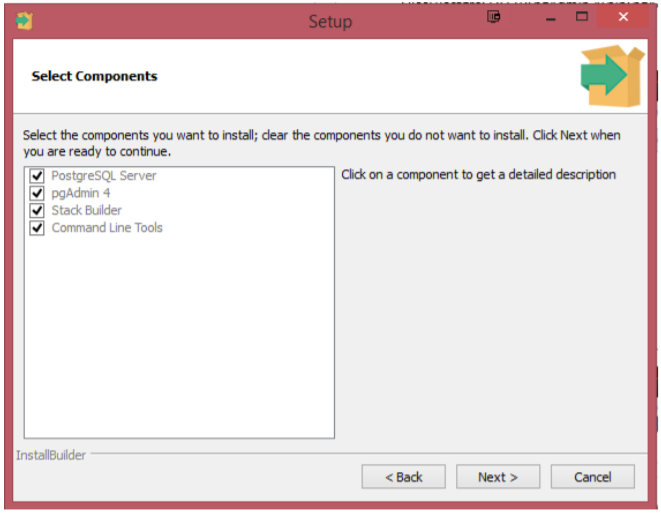
\includegraphics[scale=0.65]{Slike/Instalacija.png}
				\centering
				\caption{Odabir komponenti za instalaciju}
				\label{fig:dijagram}
			\end{figure}
			
			Zatim se unosi lozinka za administratora i odabire se port za pristup bazi podataka (defaultni port 5432). Kliknuti na "Next" kako bi započela instalacija, kada je proces instalacije završen kliknuti na "Finish". \newline
			Nakon instalacije baze podataka potrebno ju je osposobiti za BugBusters aplikaciju. Potrebno je kreirati novu praznu bazu podataka imena "bugbusters" te novog korisnika SUBP-a korisničkog imena "bugbustersUser" te lozinke "bbpassword1234" i dati mu ovlasti nad kreiranom bazom.
			\\
			 
	\textbf{Pokretanje web aplikacije}
		
		Za pokretanje web aplikacije potrebno je instalirati servlet container \underline{Tomcat 9}\footnote{\url{https://tomcat.apache.org/download-90.cgi}} inačice core. Nakon preuzimanja zip arhive s navedenog linka, raspakirajte ju. U direktorij webapps, unutar raspakiranog direktorija, potrebno je smjestiti .war datoteku objavljenu na GitLab sustavu u direktoriju "izvrsniKod". Zadnji korak je pokretanje samog servlet containera. Pozicionirajte se pomoću naredbenog retka u raspakirani direktorij u poddirektorij imena "bin". Nakon toga je potrebno izvesti naredbu "startup.bat" ukoliko se koristi Windows radno okruženje ili "startup.sh" ukoliko se koristi Unix-based radno okruženje.
		\\
	
			
		\textbf{Pokretanje android aplikacije}		
		 Mobilna android aplikacija objavljena je na F-Droid trgovini, gdje ju je moguće preuzeti i zatim instalirati na vlastiti mobilni uređaj. Spajanje na RESTful dio web poslužitelja omogućuje mobilnoj aplikaciji komunikaciju s bazom podataka i prijavu u sustav.